\appendix 
\section{Anhang A}

\subsection{Aufnahmen mit der HoloLens}
Zunächst ist festzuhalten, dass herkömmliche Bildschirmaufnahmen auf der HoloLens nur eingeschränkt sinnvoll sind. Hier wären nämlich nur die gerenderten Objekte sichtbar, die so auch in einer Entwicklungsumgebung zu sehen sind. Die Nutzererfahrung entsteht jedoch durch das Zusammenspiel mit dem Hintergrund. Deshalb bietet die HoloLens eine angepasste Funktion, um möglichst das abzubilden, was der Nutzer tatsächlich sieht: Das \textit{Mixed Reality Capture (MRC)}.\\

Mit dem Mixed Reality Capture lassen sich Screenshots und Screen-Videos aufnehmen. Dazu nutzt die Brille ihre integrierte Frontkamera und überlagert deren Bild mit dem gerenderten Bild. So lässt sich besser darstellen, was ein Nutzer sieht. Allerdings bringt dieses Vorgehen mehrere Einschränkungen mit sich, durch die die Resultate von den tatsächlich wahrgenommenen Bildern abweichen. Die wichtigsten Faktoren sind dabei:

\begin{itemize}
	\setlength{\itemsep}{-1pt}
	\singlespacing
	\item Andere Auflösung mit geringerer Pixeldichte
	\item Stark vergrößertes Sichtfeld
	\item Verfälschte Farben und Transparenzen
	\item Verfälschte Positionierung
	\item MRC nicht möglich, wenn Kamera durch Anwendung genutzt wird
\end{itemize}

Bei einem MRC-Foto ändert sich die Auflösung von 1268x720 (720p) zu 1408x792. Obwohl die Auflösung steigt ist damit dennoch ein wesentlicher Qualitätsverlust verbunden, da die höhere Auflösung des Einzelbildes nicht mit einer höheren Pixeldichte einhergeht, sondern mit einem überproportional größeren Sichtfeld. Ein Foto repräsentiert daher nicht die tatsächlichen Begrenzungen des FOV. Außerdem sinkt die Pixeldichte.\\

Dazu kommt die Transparenz von virtuellen Objekten. Diese hängt stark von deren Farbe sowie der Hintergrundhelligkeit ab und entspricht nicht immer der Wahrnehmung des Nutzers. Farbige Objekte erscheinen auf Fotos stets etwas transparent, auch wenn sie den Hintergrund aus Sicht des Nutzers vollständig überdecken. Nicht zuletzt ist auch für Fotos die Reduktion der Bildwiederholrate auf 30Hz relevant. Denn dadurch werden die Objekte nicht so gut stabilisiert und es kann zu leichten Verschiebungen auf den Fotos kommen.\\

Darüber hinaus gibt es Faktoren, die durch ein Foto nicht abgedeckt werden können. Dazu gehören die schon erläuterten Eigenheiten der stereoskopischen Wahrnehmung. Auf einem Foto sieht ein Objekt immer scharf aus und es gibt keine Probleme mit der Akkommodation oder Konvergenz, auch wenn ein Nutzer diese möglicherweise erfährt. Außerdem nimmt ein Nutzer die Umgebung anders wahr als auf einem Foto, da das Sichtfeld (auf die Umgebung) kaum eingeschränkt wird und nicht in Farbe und Auflösung begrenzt ist, sondern direkt wahrgenommen wird.\\

Diese Faktoren gilt es bei der Bewertung solcher Bilder zu berücksichtigen. Prinzipiell sind auch Aufnahmen möglich, die näher an die tatsächliche Nutzererfahrung heranreichen. Diese erfordern aber weiteres Equipment, das im Rahmen dieser Arbeit nicht zur Verfügung stand.

\subsection{Performancemessungen}
Die folgende Abbildung zeigt den Ressourcenverbrauch durch das System ohne laufende Anwendungen. Dieser wurde unmittelbar vor dem den Messungen erhoben.
\begin{figure}[h!]
	\centering
	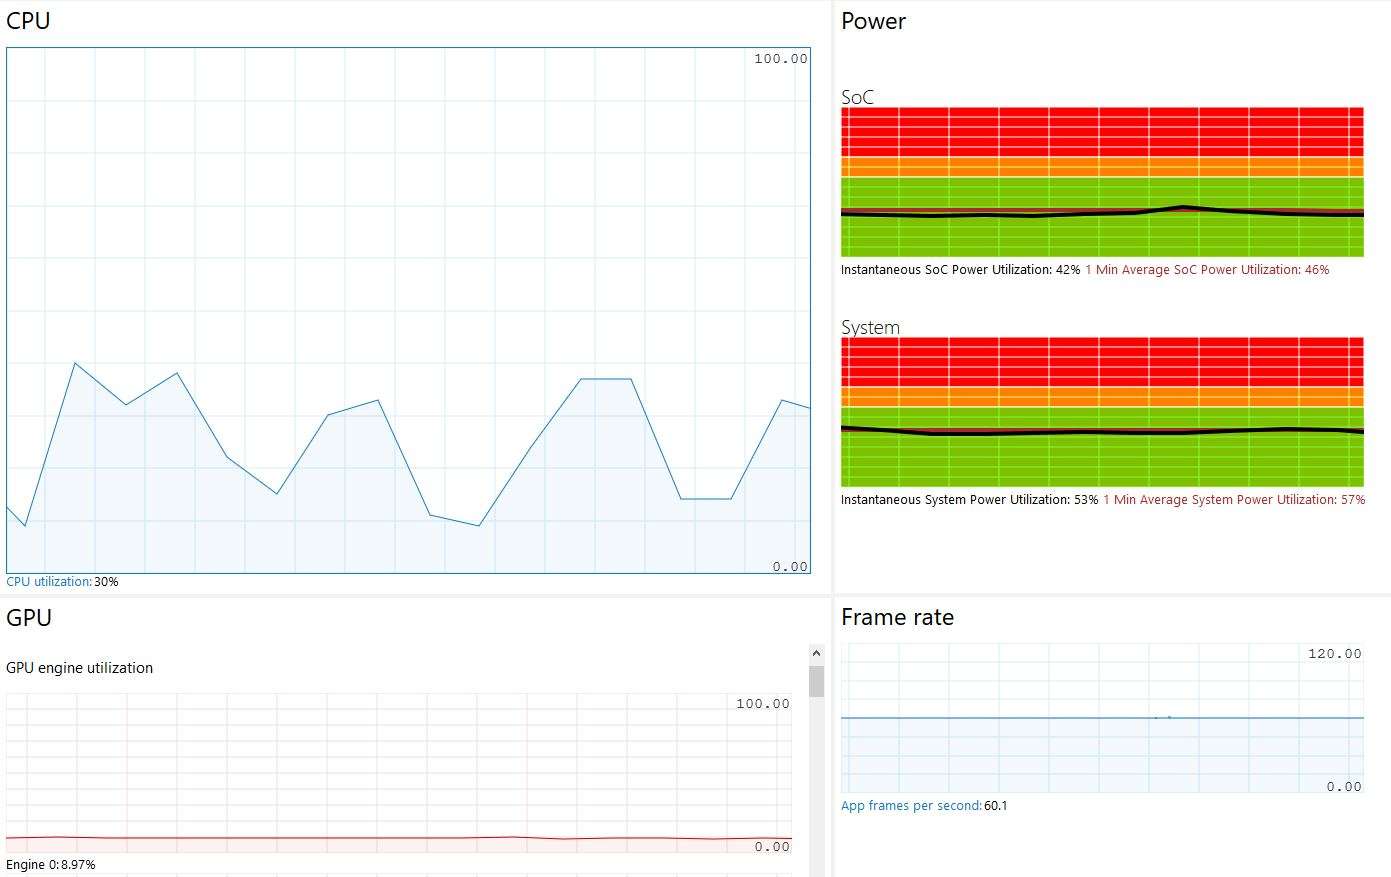
\includegraphics[width=0.8\textwidth]{images/performance/idle.jpg}
	\caption{Auslastung des Systems im Idle-Zustand.}
	\label{img:idle}
\end{figure}
